% ISPOR Europe 2026, Vienna - ML-NMR-B podium talk
% Compile with pdfLaTeX. To show speaker notes, uncomment the \setbeameroption line below.
\documentclass[aspectratio=169,10pt,t]{beamer}
 \setbeameroption{show notes on second screen=right}

\usepackage[T1]{fontenc}
\usepackage{bm}
\usepackage{microtype}
\usepackage{tikz}
\usetikzlibrary{arrows.meta,positioning,calc,shapes.geometric}
\usepackage[most]{tcolorbox}

% ---------- Fonts: Source Sans / Source Serif on Overleaf, fallbacks elsewhere ----------
\IfFileExists{sourcesanspro.sty}{\usepackage[default]{sourcesanspro}}{\usepackage{helvet}\renewcommand{\familydefault}{\sfdefault}}
\IfFileExists{sourceserifpro.sty}{\usepackage{sourceserifpro}\newcommand{\headfont}{\rmfamily}}{\newcommand{\headfont}{\fontfamily{ppl}\selectfont}}
\usefonttheme[onlymath]{serif}

% ---------- Colours ----------
\definecolor{bristolred}{HTML}{C02F38}
\definecolor{ink}{HTML}{1E1A1B}
\definecolor{body}{HTML}{4A4546}
\definecolor{muted}{HTML}{7A7173}
\definecolor{rulegrey}{HTML}{E3DDD9}
\definecolor{sand}{HTML}{F1ECE8}
\definecolor{pinkbg}{HTML}{F8E3E4}
\definecolor{randteal}{HTML}{1F6F6B}
\definecolor{tealbg}{HTML}{EEF5F4}
\definecolor{fixorange}{HTML}{A8581A}
\definecolor{orangebg}{HTML}{FBF2EA}
\definecolor{extgrey}{HTML}{7A7173}
\definecolor{studyblue}{HTML}{2F5D8C}
\definecolor{studyochre}{HTML}{C77A1A}
\definecolor{netpurple}{HTML}{B9AED6}
\definecolor{netpurpleline}{HTML}{7B68A6}
\definecolor{netgreen}{HTML}{C3DDA9}
\definecolor{netgreenline}{HTML}{86B05C}

% ---------- Theme ----------
\setbeamercolor{normal text}{fg=ink,bg=white}
\setbeamercolor{structure}{fg=bristolred}
\setbeamercolor{frametitle}{fg=ink}
\setbeamercolor{itemize item}{fg=bristolred}
\setbeamertemplate{navigation symbols}{}
\setbeamertemplate{itemize items}[circle]
\setbeamersize{text margin left=10mm,text margin right=10mm}
\hyphenpenalty=10000
\exhyphenpenalty=10000

% Frame style: "content" (red top bar + footer) or "cover" (red left bar, no footer)
\def\framestyle{content}
\setbeamertemplate{background canvas}{%
  \begin{tikzpicture}[remember picture,overlay]
    \fill[white] (current page.south west) rectangle (current page.north east);
    \def\tmp{cover}%
    \ifx\framestyle\tmp
      \fill[bristolred] (current page.north west) rectangle ([xshift=2mm]current page.south west);
    \else
      \fill[bristolred] (current page.north west) rectangle ([yshift=-1mm]current page.north east);
    \fi
  \end{tikzpicture}}

\setbeamertemplate{frametitle}{%
  \vspace*{4mm}%
  \ifx\insertframesubtitle\empty\else
    {\scriptsize\bfseries\color{bristolred}\textls[120]{\MakeUppercase{\insertframesubtitle}}\par}\vspace{1.2mm}%
  \fi
  {\headfont\LARGE\bfseries\color{ink}\insertframetitle\par}%
  \vspace{1mm}}

\newcommand{\footleft}{S. J. Perren \textperiodcentered{} University of Bristol}
\setbeamertemplate{footline}{%
  \def\tmp{cover}%
  \ifx\framestyle\tmp\else
  \hspace*{10mm}{\scriptsize\color{muted}\footleft}\hfill{\scriptsize\color{muted}\insertframenumber}\hspace*{10mm}\par\vspace*{4mm}%
  \fi}

% ---------- Helpers ----------
\newcommand{\eyebrow}[2][bristolred]{{\scriptsize\bfseries\color{#1}\textls[120]{\MakeUppercase{#2}}}}
\newcommand{\statement}[1]{{\headfont\large #1\par}}
\newcommand{\point}[2][bristolred]{%
  \begin{minipage}[t]{\linewidth}\raggedright{\color{#1}\rule{\linewidth}{1.2pt}}\par\vspace{0.8mm}{\footnotesize\color{body}#2}\end{minipage}}
\newcommand{\limitation}[1]{\begin{minipage}[t]{\linewidth}\raggedright\textcolor{bristolred}{\tikz[baseline=-0.6ex]{\draw[bristolred,line width=1.3pt,line cap=round] (-0.9mm,-0.9mm) -- (0.9mm,0.9mm) (-0.9mm,0.9mm) -- (0.9mm,-0.9mm);}}\hspace{1.5mm}{\footnotesize\color{ink}#1}\end{minipage}}
\newtcolorbox{card}[1][]{enhanced,colback=white,colframe=rulegrey,boxrule=0.7pt,arc=1.5mm,
  left=2.5mm,right=2.5mm,top=1.5mm,bottom=1.5mm,before upper={\raggedright\setlength{\parskip}{0.8mm}},#1}
\newtcolorbox{tintcard}[2][]{enhanced,colback=#2,frame hidden,arc=1.5mm,
  left=2.5mm,right=2.5mm,top=1.5mm,bottom=1.5mm,before upper={\raggedright\setlength{\parskip}{0.8mm}},#1}

\pgfmathdeclarefunction{gauss}{3}{\pgfmathparse{exp(-0.5*((#1-#2)/#3)^2)}}
\pgfmathdeclarefunction{logist}{3}{\pgfmathparse{1/(1+exp(-(#1-#2)/#3))}}
\tikzset{
  axis/.style={draw=muted!70,line width=0.6pt},
  node circ/.style={circle,draw=ink,line width=0.8pt,fill=sand,minimum size=8mm,inner sep=0pt,font=\small\bfseries},
  edge/.style={draw=body,line width=1.6pt},
  pnode/.style={circle,draw=netpurpleline,line width=0.9pt,fill=netpurple,minimum size=5mm,inner sep=0pt,font=\scriptsize\bfseries},
  gnode/.style={circle,draw=netgreenline,line width=0.9pt,fill=netgreen,minimum size=5mm,inner sep=0pt,font=\scriptsize\bfseries},
  pedge/.style={draw=netpurpleline,line width=1.1pt},
  gedge/.style={draw=netgreenline,line width=1.1pt},
  flowarrow/.style={-{Stealth[length=2.2mm]},line width=1.4pt},
  pill/.style={rounded corners=2.5mm,fill=sand,inner sep=1.4mm,font=\scriptsize\bfseries},
}

\title{Bridging disconnected networks and single-arm studies with multilevel network meta-regression}
\author{S. J. Perren, N. J. Welton, H. Pedder, D. M. Phillippo}
\institute{University of Bristol}

\begin{document}

% =====================================================================
{\def\framestyle{cover}
\begin{frame}[plain]
\vspace*{2mm}
\eyebrow{ISPOR Europe 2026 \textperiodcentered{} Vienna}
\vfill
{\headfont\Huge\bfseries\color{ink}Bridging disconnected networks and single-arm studies with multilevel network meta-regression\par}
\vspace{5mm}
{\Large\bfseries\color{bristolred}ML-NMR-B\par}
\vfill
{\normalsize S. J. Perren, N. J. Welton, H. Pedder, D. M. Phillippo\par}
\vspace{1mm}
{\footnotesize\color{muted}University of Bristol\par}
\vspace*{3mm}
\note{\textasciitilde 15 s. Hi, I'm Sam, a PhD student at Bristol. My presentation will cover, why disconnected networks in NMA are a problem, how we extended ML-NMR to bridge them.}
\end{frame}
}

\begin{frame}{Disconnected networks and single-arm studies}{The problem}
\begin{columns}[T,onlytextwidth]
\column{0.70\textwidth}
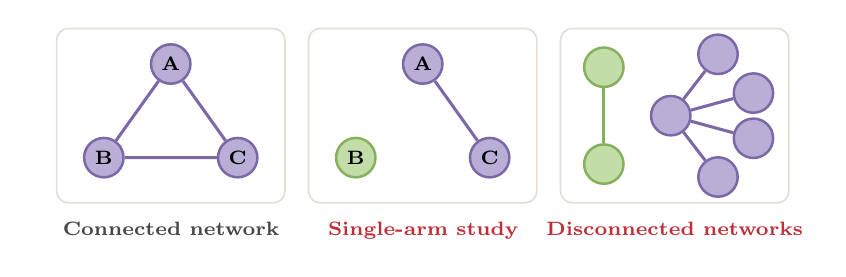
\begin{tikzpicture}[x=1mm,y=0.82mm]
  \foreach \px/\lab/\col in {0/Connected network/body, 32/Single-arm study/bristolred, 64/Disconnected networks/bristolred}
    \node[anchor=north,font=\scriptsize\bfseries,text=\col,text width=34mm,align=center] at (\px+14.5,-1.5) {\lab};
  \foreach \px in {0,32,64} \draw[rulegrey,line width=0.6pt,rounded corners=1.5mm] (\px,0) rectangle ++(29,27);
  % connected: triangle
  \node[pnode] (a1) at (14.5,21.5) {A};
  \node[pnode] (b1) at (6,7) {B};
  \node[pnode] (c1) at (23,7) {C};
  \draw[pedge] (a1) -- (b1) (a1) -- (c1) (b1) -- (c1);
  % single-arm study
  \node[pnode] (a2) at (46.5,21.5) {A};
  \node[gnode] (b2) at (38,7) {B};
  \node[pnode] (c2) at (55,7) {C};
  \draw[pedge] (a2) -- (c2);
  % disconnected sub-networks
  \node[gnode] (a3) at (69.5,21) {};
  \node[gnode] (b3) at (69.5,6) {};
  \draw[gedge] (a3) -- (b3);
  \node[pnode] (h) at (78,13.5) {};
  \foreach \xx/\yy in {84/23, 88.5/17, 88.5/10, 84/4} { \node[pnode] (t) at (\xx,\yy) {}; \draw[pedge] (h) -- (t); }
\end{tikzpicture}
\column{0.27\textwidth}\raggedright
\eyebrow[muted]{Review of NICE TAs}\par
{\tiny\color{muted}268 appraisals, 2010--18\\Phillippo et al., PharmacoEconomics 2019\par}\vspace{1mm}
{\headfont\Large\bfseries\color{bristolred}18/268}\par
{\scriptsize\color{body}used population adjustment}\par\vspace{1mm}
{\headfont\Large\bfseries\color{bristolred}16/18}\par
{\scriptsize\color{body}of those unanchored, using MAIC}\par\vspace{1mm}
{\headfont\Large\bfseries\color{bristolred}10/18}\par
{\scriptsize\color{body}involved more than two treatments}
\end{columns}
\vfill
\begin{tcolorbox}[enhanced,colback=sand,frame hidden,borderline west={1.2mm}{0mm}{bristolred},arc=1.5mm,left=4mm,right=3mm,top=1.5mm,bottom=2mm]
{\small\bfseries Limitations of MAIC and STC}\par\vspace{1.2mm}
\begin{columns}[t,onlytextwidth]
\column{0.31\textwidth}\limitation{One pair of studies at a time}
\column{0.33\textwidth}\limitation{Estimates only in the aggregate study's population}
\column{0.33\textwidth}\limitation{No way to assess whether the key assumption is plausible}
\end{columns}
\end{tcolorbox}
\vspace{1mm}
\note{\textasciitilde 1:15. Network meta-analysis lets us compare many treatments at once, as long as every treatment is joined by a path of randomised trials, like the triangle on the left. Health technology assessment committees increasingly see the other two pictures: a treatment that only comes from a single-arm study, or whole sub-networks with no common comparator between them. Comparisons across that gap are unanchored. In a review of 268 NICE appraisals from 2010 to 2018, 18 used population adjustment methods, and 16 of those were unanchored comparisons using Matching adjusted indirect comparisons (MAIC). And in over half of them, the decision involved more than two treatments, but MAIC and Simulated Treatment Comparisons (STC) can only compare one pair of studies at a time. They also only give estimates in the aggregate study's population, and give you no way to assess whether the assumption they rest on is plausible.}
\end{frame}
% =====================================================================
\begin{frame}
\vfill
\begin{columns}[c,onlytextwidth]
\column{0.66\textwidth}
\raggedright
{\large\color{body}Comparing treatments across a disconnected network assumes\par}\vspace{2mm}
{\headfont\huge\bfseries\color{bristolred}Conditional constancy of absolute effects\par}\vspace{3mm}
{\large\color{ink}Once covariates are adjusted for, absolute outcomes are exchangeable across studies.\par}\vspace{4mm}
\begin{tcolorbox}[enhanced,colback=sand,frame hidden,borderline west={1.2mm}{0mm}{bristolred},arc=1.5mm,left=4mm,right=3mm,top=1.5mm,bottom=2mm,before upper=\raggedright]
{\large\bfseries\color{ink}Every prognostic factor and effect modifier must be balanced, including unmeasured ones\par}\vspace{1.5mm}
{\footnotesize\color{body}A connected NMA only needs effect modifiers balanced, because randomisation takes care of prognostic factors. Across a disconnected network, nothing does.\par}
\end{tcolorbox}
\column{0.30\textwidth}
\centering
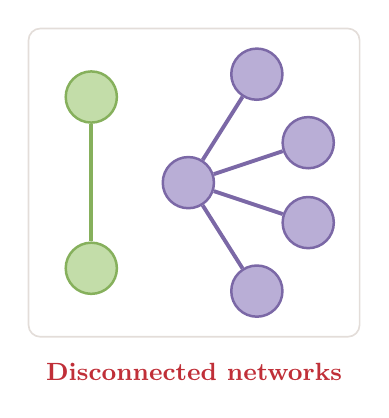
\begin{tikzpicture}[x=1.45mm,y=1.45mm]
  \draw[rulegrey,line width=0.6pt,rounded corners=1.5mm] (0,0) rectangle ++(29,27);
  \node[gnode,minimum size=6.5mm] (a3) at (5.5,21) {};
  \node[gnode,minimum size=6.5mm] (b3) at (5.5,6) {};
  \draw[gedge,line width=1.4pt] (a3) -- (b3);
  \node[pnode,minimum size=6.5mm] (h) at (14,13.5) {};
  \foreach \xx/\yy in {20/23, 24.5/17, 24.5/10, 20/4} { \node[pnode,minimum size=6.5mm] (t) at (\xx,\yy) {}; \draw[pedge,line width=1.4pt] (h) -- (t); }
  \node[anchor=north,font=\small\bfseries,text=bristolred] at (14.5,-1.5) {Disconnected networks};
\end{tikzpicture}
\end{columns}
\vfill
\note{\textasciitilde 0:45. Whatever method you use, comparing treatments across a disconnected network rests on the assumption of conditional constancy of absolute effects. Once you've adjusted for covariates, absolute outcomes are exchangeable between studies. The key word is absolute. A connected NMA only assumes constancy of relative effects, so only effect modifiers need to be balanced, and randomisation takes care of prognostic factors. Across a disconnected network there's no randomisation to lean on, so every prognostic factor and effect modifier has to be balanced or adjusted for, including the ones we can't measure.}
\end{frame}

% =====================================================================
\begin{frame}{ML-NMR: one model for IPD and aggregate data}{Population adjustment}
\begin{columns}[T,onlytextwidth]
\column{0.485\textwidth}
\begin{card}
\eyebrow{Studies with IPD: fit to individuals}

\centering
\begin{tikzpicture}[x=1mm,y=1mm]
  \draw[axis] (0,0) -- (58,0);
  \draw[bristolred,line width=1.4pt,domain=0:58,samples=60] plot (\x,{2+16*logist(\x,30,5)});
  \foreach \x in {3,7,11,15,18,21,25,32} \fill[ink,opacity=0.55] (\x,2) circle (0.9);
  \foreach \x in {26,33,36,40,44,48,52,56} \fill[ink,opacity=0.55] (\x,18) circle (0.9);
\end{tikzpicture}

\raggedright
{\scriptsize\color{body}Each dot is one person: responded (top) or not (bottom), by covariate value}

\centering
$\eta_{jk}(\bm{x}) = \mu_j + \bm{x}^T(\bm{\beta}_1 + \bm{\beta}_{2k}) + \gamma_k$
\end{card}
\column{0.485\textwidth}
\begin{card}
\eyebrow{Aggregate data: integrate over $f(\bm{x})$}

\centering
\begin{tikzpicture}[x=1mm,y=1mm]
  \draw[axis] (0,0) -- (58,0);
  \fill[bristolred,opacity=0.15,domain=8:52,samples=50] plot (\x,{14*gauss(\x,30,7)}) -- (52,0) -- (8,0) -- cycle;
  \draw[bristolred,opacity=0.6,line width=1pt,domain=8:52,samples=50] plot (\x,{14*gauss(\x,30,7)});
  \draw[ink,line width=1.4pt,domain=0:58,samples=60] plot (\x,{2+16*logist(\x,30,5)});
\end{tikzpicture}

\raggedright
{\scriptsize\color{body}Shaded: the study's covariate distribution, from its reported summaries}

\centering
$\theta_{\bullet jk} = \displaystyle\int g^{-1}\{\eta_{jk}(\bm{x})\}\, f_{jk}(\bm{x})\, d\bm{x}$
\end{card}
\end{columns}
\vfill
\statement{Any network size, any target population. \textcolor{bristolred}{But only for connected networks.}}
\vspace{2mm}
\note{\textasciitilde 1:00. So first how do we get the conditional part of this assumption. The tool we use to adjust is ML-NMR. For studies with IPD we fit an individual-level regression: a study baseline mu, prognostic effects beta-1, effect modifiers beta-2, and treatment effects gamma. For studies with only aggregate data, we take that same individual model and integrate it over the study's covariate distribution, so there's no aggregation bias. That gives population adjustment in networks of any size, with estimates in whatever target population the decision needs. But until now it needed a connected network.}
\end{frame}

% =====================================================================
\begin{frame}{Bridge the gap through the study baselines}{The idea}
\begin{columns}[c,onlytextwidth]
\column{0.58\textwidth}
\centering
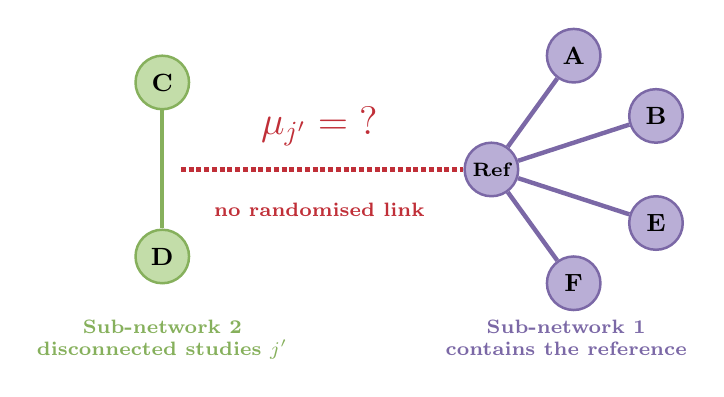
\begin{tikzpicture}[x=0.95mm,y=0.85mm,
    bigp/.style={pnode,minimum size=6.8mm,font=\small\bfseries},
    bigg/.style={gnode,minimum size=6.8mm,font=\small\bfseries}]
  % sub-network 2 (disconnected): green pair
  \node[bigg] (c) at (10,30) {C};
  \node[bigg] (d) at (10,4) {D};
  \draw[gedge,line width=1.6pt] (c) -- (d);
  % sub-network 1 (reference)
  \node[bigp,font=\scriptsize\bfseries] (ref) at (54,17) {Ref};
  \foreach \xx/\yy/\lab in {65/34/A, 76/25/B, 76/9/E, 65/0/F} {
    \node[bigp] (t) at (\xx,\yy) {\lab}; \draw[pedge,line width=1.6pt] (ref) -- (t); }
  % the bridge
  \draw[bristolred,densely dotted,line width=1.8pt] (12.5,17) -- (ref);
  \node[font=\Large,text=bristolred] at (31,23.5) {$\mu_{j'} = {?}$};
  \node[font=\scriptsize\bfseries,text=bristolred] at (31,11) {no randomised link};
  % labels
  \node[anchor=north,font=\scriptsize\bfseries,text=netgreenline,align=center] at (10,-4) {Sub-network 2\\disconnected studies $j'$};
  \node[anchor=north,font=\scriptsize\bfseries,text=netpurpleline,align=center] at (64,-4) {Sub-network 1\\contains the reference};
\end{tikzpicture}
\column{0.38\textwidth}
\raggedright
{\small\color{body}Relative effects within sub-network 2 still come from its own trials. Covariate effects are shared across the network.\par}\vspace{4mm}
{\small\color{body}\textcolor{bristolred}{\textbf{Missing:}} $\mu_{j'}$, the outcome on the reference treatment in the disconnected studies.\par}\vspace{4mm}
{\small\color{ink}\textbf{Single-arm studies} are bridged the same way.\par}\vspace{4mm}
{\scriptsize\color{muted}Builds on models for baselines across studies (B\'eliveau et al.\ 2017; Thom et al.\ 2022).\par}
\end{columns}
\vfill
\centering
{\Large $\eta_{j'k}(\bm{x}) = \colorbox{pinkbg}{$\color{bristolred}\mu_{j'}$} + \bm{x}^T(\bm{\beta}_1 + \bm{\beta}_{2k}) + \gamma_k$}\par
\vspace{4mm}
\note{\textasciitilde 0:50. Here's the idea. Sub-network 1, in purple, has the reference treatment. That's usually placebo, but any well-informed treatment will do. Sub-network 2, in green, has no randomised path to that reference. If we look at the linear predictor, relative effects within sub-network 2 still come from its own trials, and the covariate effects are shared across the whole network. What's missing is mu j-prime, the study baseline: the adjusted outcome on the reference treatment in those studies, which they can't tell us because the reference isn't observed there. That's the one thing we provide to this disconnected part. If there is IPD within either subnetwork, we can add individual-level adjustment, and we call this ML-NMR with bridging, ML-NMR-B. A single-arm study is bridged in the same way. There are two methods to ML-NMR-B.}
\end{frame}

% =====================================================================
\begin{frame}{The random baseline bridge, in two stages}{Bridge 1 \textperiodcentered{} preferred where data allow}
\centering
\begin{tikzpicture}[x=1mm,y=1mm,
    sp/.style={pnode,minimum size=4.6mm},
    sg/.style={gnode,minimum size=4.6mm}]
  \fill[tealbg,rounded corners=1.5mm] (0,0) rectangle (64,51);
  \fill[tealbg,rounded corners=1.5mm] (76,0) rectangle (140,51);
  \draw[randteal,flowarrow] (65.5,27) -- (74.5,27);
  \node[font=\tiny\bfseries,text=randteal,align=center,anchor=south] at (70,28) {$\mu_\mathrm{new}$\\only};
  % ---------------- Stage 1 ----------------
  \node[anchor=north west,align=left,text width=59mm] at (2.5,49.5) {\eyebrow[randteal]{Stage 1 \textperiodcentered{} baseline synthesis}\\[0.6mm]{\footnotesize\bfseries All studies fitted together, with a random effect on the reference baselines}};
  \node[sg] (c1) at (12,32.5) {}; \node[sg] (d1) at (12,18) {}; \draw[gedge] (c1) -- (d1);
  \node[sp,minimum size=6mm,font=\tiny\bfseries] (h1) at (40,25) {Ref};
  \foreach \xx/\yy in {47/33, 53/28.5, 53/21.5, 47/17} { \node[sp] (t) at (\xx,\yy) {}; \draw[pedge] (h1) -- (t); }
  \draw[randteal,line width=1.3pt] (h1) circle (4.6mm);
  \node[font=\tiny\bfseries,text=randteal,anchor=east] at (34.5,29.5) {random effect};
  % baseline distribution -> predictive
  \draw[axis] (3,8) -- (29,8);
  \draw[randteal,line width=1.1pt,domain=3:29,samples=40] plot (\x,{8+7*gauss(\x,16,3.2)});
  \foreach \x in {12.5,15,17.5,20} \fill[netpurpleline] (\x,8) circle (0.8);
  \draw[randteal,-{Stealth[length=1.6mm]},line width=0.9pt] (30,11) -- (35,11);
  \fill[randteal,opacity=0.25,domain=36:62,samples=40] plot (\x,{8+5*gauss(\x,49,4.8)}) -- (62,8) -- (36,8) -- cycle;
  \draw[randteal,line width=1.1pt,domain=36:62,samples=40] plot (\x,{8+5*gauss(\x,49,4.8)});
  \draw[axis] (36,8) -- (62,8);
  \node[font=\scriptsize] at (16,3.5) {$\mu_j \sim N(m_\mu, \tau_\mu^2)$};
  \node[font=\scriptsize] at (49,3.5) {predictive $\mu_\mathrm{new}$};
  % ---------------- Stage 2 ----------------
  \node[anchor=north west,align=left,text width=59mm] at (78.5,49.5) {\eyebrow[randteal]{Stage 2 \textperiodcentered{} the bridge}\\[0.6mm]{\footnotesize\bfseries Prior on the disconnected baselines}};
  \node[sg,minimum size=6mm] (c2) at (85,36.5) {}; \node[sg,minimum size=6mm] (d2) at (85,20.5) {}; \draw[gedge,line width=1.3pt] (c2) -- (d2);
  \node[sp,minimum size=6mm,font=\tiny\bfseries] (h2) at (121,28.5) {Ref};
  \foreach \xx/\yy in {128/37, 134/32.5, 134/24.5, 128/20} { \node[sp] (t) at (\xx,\yy) {}; \draw[pedge] (h2) -- (t); }
  \draw[bristolred,densely dotted,line width=1.5pt] (87,28.5) -- (h2);
  \fill[randteal,opacity=0.25,domain=92:112,samples=40] plot (\x,{30+6*gauss(\x,102,3.6)}) -- (112,30) -- (92,30) -- cycle;
  \draw[randteal,line width=1.1pt,domain=92:112,samples=40] plot (\x,{30+6*gauss(\x,102,3.6)});
  \node[font=\scriptsize,text=ink] at (102,24) {$\mu_{j'} \sim \pi(\mu_\mathrm{new})$};
  \node[anchor=north west,text width=59mm,align=left,font=\scriptsize,text=body] at (78.5,15) {Only the disconnected studies get the prior. Randomised comparisons within each sub-network stay untouched.};
\end{tikzpicture}
\vfill
\raggedright
\statement{Assumes the adjusted baselines of all bridged studies are exchangeable.}
\vspace{2mm}
\note{\textasciitilde 1:15. First is the random baseline bridge, which has two stages. Stage 1, on the left, fits ML-NMR to all the studies together, but puts a random effect on the network reference treatment. Every study contributes to that: the reference studies directly, and the others through the shared covariate effects. For this treatment, that gives a mean and a between-study SD, tau-mu, the variation left after adjusting for covariates, and from those a predictive distribution for the baseline in a new study, mu new. That's the only thing we carry forward into Stage 2, on the right: that predictive distribution sits on the bridge as an informative prior on the baselines of the disconnected studies only. By running it in two stages, we preserve the randomisation within each sub-network. And by using the predictive distribution as a prior, we propagate uncertainty about unmeasured prognostic factors into the estimates for the disconnected studies. It assumes the adjusted baselines of all bridged studies are exchangeable, and because some unobserved differences between studies are almost always there, we prefer this bridge where the data allow.}
\end{frame}

% =====================================================================
\begin{frame}{The fixed baseline bridge: merge an anchor pair}{Bridge 2}
\centering
\begin{tikzpicture}[x=1mm,y=1mm,
    sp/.style={pnode,minimum size=4.6mm},
    sg/.style={gnode,minimum size=4.6mm}]
  \fill[orangebg,rounded corners=1.5mm] (0,0) rectangle (64,51);
  \fill[orangebg,rounded corners=1.5mm] (76,0) rectangle (140,51);
  \draw[fixorange,flowarrow] (65.5,27) -- (74.5,27);
  % ---------------- Step 1 ----------------
  \node[anchor=north west,align=left,text width=59mm] at (2.5,49.5) {\eyebrow[fixorange]{Step 1 \textperiodcentered{} pick an anchor pair}\\[0.6mm]{\footnotesize\bfseries One study from each sub-network}};
  % anchor halos
  \draw[fixorange,opacity=0.45,line width=6pt,line cap=round] (9,36.5) -- (9,20.5);
  \draw[fixorange,opacity=0.45,line width=6pt,line cap=round] (34,28.5) -- (41,20);
  \node[sg,minimum size=6mm] (c) at (9,36.5) {}; \node[sg,minimum size=6mm] (d) at (9,20.5) {}; \draw[gedge,line width=1.3pt] (c) -- (d);
  \node[sp,minimum size=6mm,font=\tiny\bfseries] (h) at (34,28.5) {Ref};
  \foreach \xx/\yy in {41/37, 47/32.5, 47/24.5, 41/20} { \node[sp] (t) at (\xx,\yy) {}; \draw[pedge] (h) -- (t); }
  \node[font=\small\bfseries,text=fixorange] at (3.5,28.5) {$j'$};
  \node[font=\small\bfseries,text=fixorange] at (45.5,17) {$j$};
  \node[anchor=north west,text width=59mm,align=left,font=\scriptsize,text=body] at (2.5,14) {Chosen as the most similar pair of populations (next slide). Can be an internal trial or an external single-arm study.};
  % ---------------- Step 2 ----------------
  \node[anchor=north west,align=left,text width=59mm] at (78.5,49.5) {\eyebrow[fixorange]{Step 2 \textperiodcentered{} share one baseline}\\[0.6mm]{\footnotesize\bfseries The pair becomes one four-arm study}};
  % combined four-arm study: cross links
  \draw[bristolred,line width=1.3pt] (85,36.5) -- (110,28.5) (85,36.5) -- (117,20) (85,20.5) -- (110,28.5) (85,20.5) -- (117,20);
  % anchor halos
  \draw[fixorange,opacity=0.45,line width=6pt,line cap=round] (85,36.5) -- (85,20.5);
  \draw[fixorange,opacity=0.45,line width=6pt,line cap=round] (110,28.5) -- (117,20);
  \node[sg,minimum size=6mm] (c) at (85,36.5) {}; \node[sg,minimum size=6mm] (d) at (85,20.5) {}; \draw[gedge,line width=1.3pt] (c) -- (d);
  \node[sp,minimum size=6mm,font=\tiny\bfseries] (h) at (110,28.5) {Ref};
  \foreach \xx/\yy in {117/37, 123/32.5, 123/24.5, 117/20} { \node[sp] (t) at (\xx,\yy) {}; \draw[pedge] (h) -- (t); }
  \node[font=\small\bfseries,text=fixorange] at (79.5,28.5) {$j'$};
  \node[font=\small\bfseries,text=fixorange] at (121.5,17) {$j$};
  \node[font=\small,text=bristolred] at (98,38) {$\mu_j = \mu_{j'}$};
  \node[anchor=north west,text width=59mm,align=left,font=\scriptsize,text=body] at (78.5,14) {Needed when only one study informs the reference, so $\tau_\mu$ can't be estimated. No extra uncertainty for unobserved differences.};
\end{tikzpicture}
\vfill
\raggedright
\statement{Assumes the pair's adjusted baselines are identical.}
\vspace{2mm}
\note{\textasciitilde 0:45. The fixed baseline bridge is simpler. Step 1: pick one anchor study from each side, highlighted in orange: j prime in the disconnected part and j in the reference part, chosen as the most similar pair of populations. I'll show how we measure that on the next slide. Step 2: give them a single shared baseline, mu j equals mu j prime, so after adjusting for the covariates they're modelled as one four-arm study, which is what the red lines show. It assumes the pair's adjusted baselines are identical, so it carries no extra uncertainty for unobserved differences. It's what you need when only one study informs the reference sub-network, so tau-mu can't be estimated. The bridge can be made with internal trials or using an external single-arm or observational study and adding it to another trail, as if it where another arm in the study. Where both the random and the fixed bridges can be fitted to a network, we use the random bridge as the main analysis and fixed bridges as sensitivity analyses.}
\end{frame}

% =====================================================================
\newcommand{\priorcurve}{\draw[muted!80,dashed,line width=0.9pt,domain=0:38,samples=50] plot (\x,{7*gauss(\x,0,20)});}
\begin{frame}{Is the bridge plausible?}{Judging the assumption}
\begin{tcbraster}[raster columns=3,raster equal height,raster column skip=3mm]
\begin{card}
\eyebrow{Overlap ESS\%}

{\small\bfseries How similar are two populations?\par}
\vspace{1mm}
\centering
\begin{tikzpicture}[x=0.6mm,y=0.75mm]
  \fill[studyblue,opacity=0.25,domain=0:30,samples=40] plot (\x,{9*gauss(\x,15,4.4)}) -- (30,0) -- (0,0) -- cycle;
  \draw[studyblue,line width=1pt,domain=0:30,samples=40] plot (\x,{9*gauss(\x,15,4.4)});
  \fill[studyochre,opacity=0.25,domain=0:30,samples=40] plot (\x,{8*gauss(\x,16.3,4.8)}) -- (30,0) -- (0,0) -- cycle;
  \draw[studyochre,line width=1pt,dashed,domain=0:30,samples=40] plot (\x,{8*gauss(\x,16.3,4.8)});
  \draw[axis] (0,0) -- (30,0);
  \node[font=\tiny\bfseries,below] at (15,0) {high overlap};
  \begin{scope}[xshift=21mm]
  \fill[studyblue,opacity=0.25,domain=0:30,samples=40] plot (\x,{9*gauss(\x,9.7,3.3)}) -- (30,0) -- (0,0) -- cycle;
  \draw[studyblue,line width=1pt,domain=0:30,samples=40] plot (\x,{9*gauss(\x,9.7,3.3)});
  \fill[studyochre,opacity=0.25,domain=0:30,samples=40] plot (\x,{8*gauss(\x,20.3,3.7)}) -- (30,0) -- (0,0) -- cycle;
  \draw[studyochre,line width=1pt,dashed,domain=0:30,samples=40] plot (\x,{8*gauss(\x,20.3,3.7)});
  \draw[axis] (0,0) -- (30,0);
  \node[font=\tiny\bfseries,below] at (15,0) {low overlap};
  \end{scope}
\end{tikzpicture}
\raggedright

{\scriptsize\color{body}Can we tell which study each person came from? Picks the anchor.\par}
{\scriptsize\color{body}\textcolor{bristolred}{\textbf{Shows how far we extrapolate,}} not whether that extrapolation is valid.\par}
\end{card}
\begin{card}
\eyebrow{Baseline variation}

{\small\bfseries $\tau_\mu$: do adjusted baselines still vary?\par}
\vspace{1mm}
\centering
\begin{tikzpicture}[x=1mm,y=0.75mm]
  \draw[axis] (0,0) -- (38,0);
  \priorcurve
  \draw[randteal,line width=1.3pt,domain=0:38,samples=60] plot (\x,{9*gauss(\x,5,2.5)});
  \draw[bristolred,line width=1.3pt,domain=0:38,samples=60] plot (\x,{9*gauss(\x,27,2.8)});
  \node[font=\tiny\bfseries,text=randteal,below] at (5,0) {reassuring};
  \node[font=\tiny\bfseries,text=bristolred,below] at (27,0) {warning};
\end{tikzpicture}
\raggedright

{\scriptsize\color{body}Best measure of unobserved differences: NMA studies already share a PICO.\par}
{\scriptsize\color{body}Posterior hugs the prior (dashed)? Too few studies to tell.\par}
\end{card}
\begin{card}
\eyebrow{Prediction}

{\small\bfseries Can the model predict well?\par}
\vspace{1mm}
\begin{itemize}\setlength{\itemsep}{1.2mm}\scriptsize
\item Leave-one-out CV in the IPD studies
\item Are covariates informative about outcomes?
\item Well estimated enough to predict into disconnected studies and target populations?
\end{itemize}
\end{card}
\end{tcbraster}
\vfill
\raggedright
\statement{None tests the assumption. With sensitivity analyses, they help judge it.}
\vspace{2mm}
\note{\textasciitilde 1:15. The assumption of conditional constancy of absolute effects can't be tested directly, but three things help us judge it. First, propensity score overlap. We pool the IPD with pseudo-IPD from the aggregate data and model which study each person came from. If the model can't tell, like the left-hand picture, overlap is high. We assume that populations that look alike on what we measured are more likely to be alike on what we didn't, accompanied with clinical input, so that's how we pick the anchor studies. It also tells you how far the model is extrapolating, but not whether that extrapolation is valid. Second, tau-mu from Stage 1: the variation left in the reference baselines after adjustment. Studies in an NMA already share a PICO and a reason to be combined, so it's our best measure of unobserved differences across the bridge. Small and precise is reassuring, large is a warning, and if the posterior just hugs the prior there aren't enough studies to tell. Third, predictive performance: leave-one-out cross-validation in the IPD studies checks the covariates are informative and the model is well estimated enough to predict into the disconnected studies and target populations. None of these tests the assumption, so we also fit several bridges as sensitivity analyses and report how much robust the estimations are.}
\end{frame}

% =====================================================================
\newcommand{\bridgetag}[3]{\begin{tcolorbox}[enhanced,colback=#1,frame hidden,borderline west={1.2mm}{0mm}{#2},arc=1mm,left=2.5mm,right=1mm,top=1mm,bottom=1mm,fontupper=\scriptsize,before upper=\raggedright]#3\end{tcolorbox}}
{\renewcommand{\footleft}{Data: Phillippo et al.\ 2023; IPD simulated to resemble the trials \textperiodcentered{} \%: overlap ESS of the anchor pair}
\begin{frame}{Psoriasis: break a network, rebuild it}{Case study}
\begin{columns}[c,onlytextwidth]
\column{0.29\textwidth}
\centering
\begin{minipage}[b][32mm][b]{\linewidth}\centering
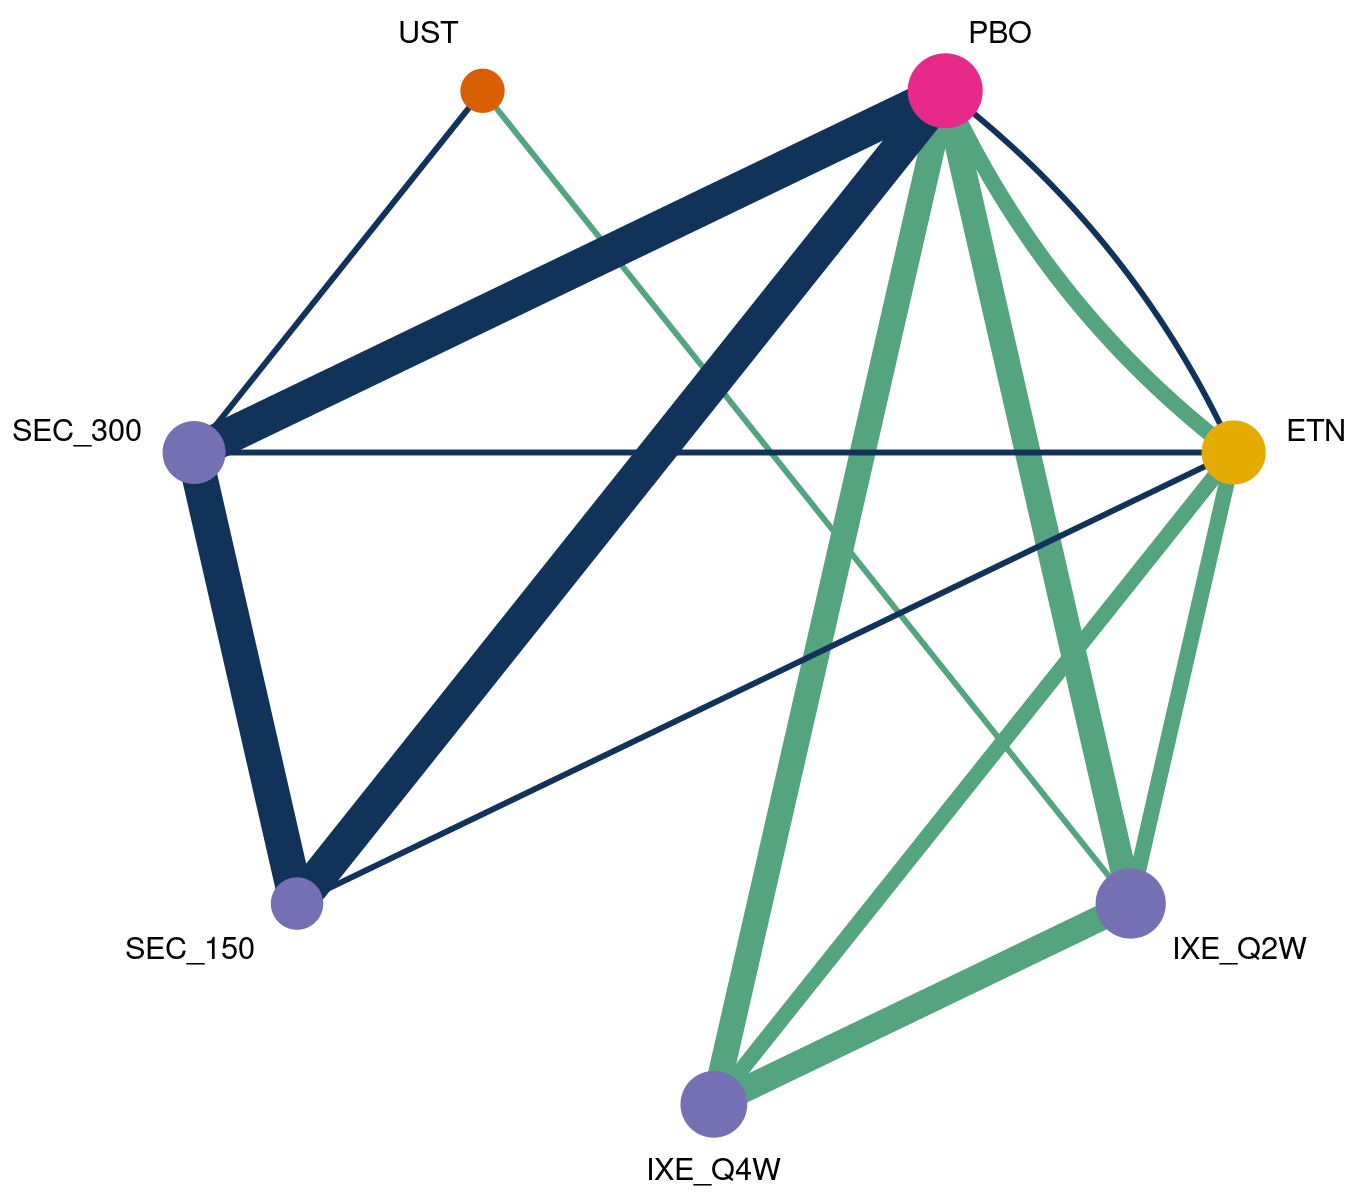
\includegraphics[width=\linewidth,height=31mm,keepaspectratio]{figures/network_full.png}
\end{minipage}\par\vspace{1mm}
{\scriptsize\bfseries Fully connected (benchmark)}
\column{0.05\textwidth}
\centering\tikz\draw[bristolred,flowarrow] (0,0) -- (5mm,0);
\column{0.29\textwidth}
\centering
\begin{minipage}[b][32mm][b]{\linewidth}\centering
\begin{tikzpicture}
  \node[inner sep=0,anchor=south west] (img) at (0,0) {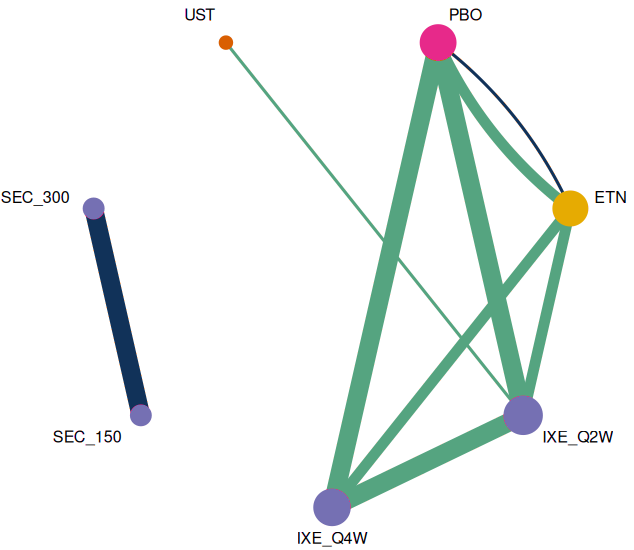
\includegraphics[width=\linewidth,height=31mm,keepaspectratio]{figures/network_disconnected.png}};
  \begin{scope}[x={(img.south east)},y={(img.north west)}]
    \node[draw=muted,fill=white,rounded corners=1mm,inner sep=0.8mm,font=\tiny\bfseries,align=center] at (0.13,0.80) {Sub-network 2\\(disconnected)};
    \node[draw=muted,fill=white,rounded corners=1mm,inner sep=0.8mm,font=\tiny\bfseries,align=center,anchor=south] at (0.68,1.01) {Sub-network 1 (reference)};
  \end{scope}
\end{tikzpicture}
\end{minipage}\par\vspace{1mm}
{\scriptsize\bfseries\color{bristolred}Artificially disconnected}
\column{0.33\textwidth}
\begin{itemize}\setlength{\itemsep}{1mm}\footnotesize
\item 9 RCTs: 4 IPD, 5 AgD
\item 6 active treatments and placebo
\item PASI 75/90/100 at 12 weeks
\item Secukinumab cut off from PBO
\item Each bridge vs the full network
\end{itemize}
\end{columns}
\vfill
\begin{tcbraster}[raster columns=3,raster equal height,raster column skip=2.5mm,raster row skip=1.5mm]
\bridgetag{tealbg}{randteal}{\textbf{Random-1P} \textperiodcentered{} prior on ERASURE}
\bridgetag{orangebg}{fixorange}{\textbf{Fixed} \textperiodcentered{} UNC-3 + ERA (97\%)}
\bridgetag{sand}{extgrey}{\textbf{Single-arm} \textperiodcentered{} PROSPECT (89\%)}
\bridgetag{tealbg}{randteal}{\textbf{Random-3P} \textperiodcentered{} prior on all three}
\bridgetag{orangebg}{fixorange}{\textbf{Fixed} \textperiodcentered{} JUNC + IXOR (74\%)}
\bridgetag{sand}{extgrey}{\textbf{Single-arm} \textperiodcentered{} Chiricozzi (77\%)}
\end{tcbraster}

\note{\textasciitilde 1:00. We did a case study of these methods on a plaque psoriasis network: nine RCTs, six active treatments plus placebo, four with IPD and five with aggregate data, with varying PASI outcomes. We kept the full network ands its estimations as our gold-standard to compare to. Then we disconnected this network to have 2 subnetworks and then we bridged these subnetworks in six ways. Two random bridges, with the predictive prior on one or all three disconnected studies. Two fixed bridges between trials: the highest-overlap pair at 97\%, and a lower one at 74\%. And two fixed bridges by combining single-arm observational studies of secukinumab, PROSPECT and Chiricozzi, onto studies as an additional arm to bridge the network. Each is compared with the fully connected ML-NMR.}
\end{frame}
}

% =====================================================================
% Forest plot: probability of PASI 75, FIXTURE population, ML-NMR (Appendix Table A3)
\newcommand{\forestpanel}[3]{% #1 x-offset (cm), #2 title, #3 list of mean/lo/hi/colour
  \begin{scope}[xshift=#1cm]
    \node[anchor=south west,font=\small\bfseries,align=left,text width=4.6cm] at (0,0.15) {#2};
    \foreach \fm/\flo/\fhi/\fc [count=\i] in {#3} {
      \ifnum\i=1
        \fill[ink,opacity=0.08] ({(\flo-0.3)/0.7*4.6},-0.05) rectangle ({(\fhi-0.3)/0.7*4.6},-2.98);
        \draw[ink,dashed,line width=0.6pt] ({(\fm-0.3)/0.7*4.6},-0.05) -- ({(\fm-0.3)/0.7*4.6},-2.98);
      \fi
      \draw[\fc,line width=1.6pt,line cap=round] ({(\flo-0.3)/0.7*4.6},-0.42*\i+0.21) -- ({(\fhi-0.3)/0.7*4.6},-0.42*\i+0.21);
      \fill[\fc] ({(\fm-0.3)/0.7*4.6},-0.42*\i+0.21) circle (0.9mm);
    }
    \draw[axis] (0,-3.0) -- (4.6,-3.0);
    \foreach \t in {0.4,0.6,0.8,1.0} {
      \draw[axis] ({(\t-0.3)/0.7*4.6},-3.0) -- ++(0,-0.08);
      \node[font=\scriptsize,text=muted,below] at ({(\t-0.3)/0.7*4.6},-3.05) {\t};
    }
  \end{scope}}
{\renewcommand{\footleft}{ML-NMR posterior mean and 95\% CrI \textperiodcentered{} dashed line and band: fully connected estimate}
\begin{frame}{Only bridged comparisons depend on the bridge}{Results \textperiodcentered{} probability of PASI 75, FIXTURE population}
\centering
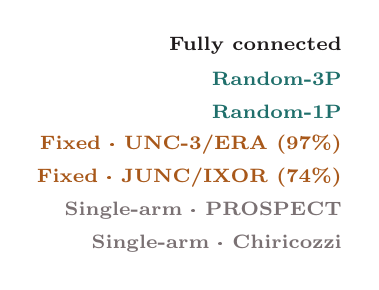
\begin{tikzpicture}
  \foreach \lab/\lc [count=\i] in {Fully connected/ink, Random-3P/randteal, Random-1P/randteal,
      {Fixed \textperiodcentered{} UNC-3/ERA (97\%)}/fixorange, {Fixed \textperiodcentered{} JUNC/IXOR (74\%)}/fixorange,
      Single-arm \textperiodcentered{} PROSPECT/extgrey, Single-arm \textperiodcentered{} Chiricozzi/extgrey}
    \node[anchor=east,font=\scriptsize\bfseries,text=\lc] at (-0.2,-0.42*\i+0.21) {\lab};
  \forestpanel{0}{Secukinumab 150 mg\\{\scriptsize\color{bristolred}crosses the bridge}}{0.67/0.63/0.70/ink, 0.66/0.56/0.76/randteal, 0.65/0.50/0.78/randteal, 0.61/0.54/0.68/fixorange, 0.66/0.54/0.78/fixorange, 0.59/0.46/0.70/extgrey, 0.50/0.37/0.62/extgrey}
  \forestpanel{5.4}{Etanercept\\{\scriptsize\color{muted}within sub-network 1}}{0.44/0.40/0.49/ink, 0.45/0.41/0.50/randteal, 0.45/0.41/0.50/randteal, 0.45/0.41/0.50/fixorange, 0.45/0.41/0.50/fixorange, 0.45/0.40/0.50/extgrey, 0.45/0.41/0.50/extgrey}
\end{tikzpicture}
\vfill
\begin{columns}[t,onlytextwidth]
\column{0.235\textwidth}\point[ink]{Etanercept: every bridge matches the full network}
\column{0.235\textwidth}\point[randteal]{Random-3P sits closest; 1P is wider}
\column{0.235\textwidth}\point[fixorange]{74\% pair as close as 97\%: overlap $\neq$ bias}
\column{0.235\textwidth}\point[extgrey]{PROSPECT overlaps, Chiricozzi drifts low}
\end{columns}
\vspace{1mm}

\note{\textasciitilde 1:30. We have two sets of results, both predicted in one of the populations FIXTURE as probability of PASI 75. The dashed line and grey band are the fully connected answer we're trying to recover. On the right is a control: etanercept, which sits inside sub-network 1, so its comparisons never cross the bridge. Every bridge gives the same answer as the full network because we havent had to use the bridge for this estimate. On the left is secukinumab 150, which does cross the bridge, and now the choice matters. The random bridge with the prior on all three disconnected studies sits closest to the connected answer, and putting the prior on one study widens the intervals, as you'd expect. The fixed bridges: the 97\% pair is more precise but shifted, while the 74\% pair recovers the connected estimate. This comparison between the fixed bridges shows that ESS\% doesnt measure for bias, both have high ESS\% overlap and are adjusted, so what's left is unobserved differences. The single-arm bridges: PROSPECT is wider and a little low, but still overlaps the connected answer, while Chiricozzi drifts furthest, most likely from unobserved differences again. The same pattern of results holds for secukinumab 300 and for PASI 90 and 100.}
\end{frame}
}

% =====================================================================
\newcommand{\takeaway}[3]{%
  {\color{rulegrey}\rule{\linewidth}{0.8pt}}\par\vspace{1.5mm}
  \begin{minipage}[t]{8mm}{\headfont\huge\bfseries\color{bristolred}#1}\end{minipage}%
  \begin{minipage}[t]{\dimexpr\linewidth-8mm}\raggedright{\large\bfseries #2}\par\vspace{0.5mm}{\footnotesize\color{body}#3}\end{minipage}\par\vspace{1mm}}
\renewcommand{\footleft}{Implemented in multinma: coming to CRAN shortly}
\begin{frame}{What ML-NMR-B gives you}{Take-homes}
\vspace*{-3mm}
\takeaway{1}{Population adjustment across disconnected networks and single-arm studies}{Builds on models for baselines (B\'eliveau 2017; Thom 2022), adding IPD-level adjustment and a two-stage fit.}
\takeaway{2}{Allows for unobserved differences}{The random baseline bridge carries residual between-study variation through as uncertainty.}
\takeaway{3}{Makes the key assumption judgeable}{$\tau_\mu$, overlap ESS and predictive checks, plus sensitivity analyses across bridges.}
\begin{tintcard}{tealbg}
{\footnotesize\textcolor{randteal}{\textbf{Next: a simulation study}}\textcolor{body}{\ will test the bias and coverage of each bridging strategy, including when the bridging assumptions fail.}\par}
\end{tintcard}
\note{\textasciitilde 0:45. Three things to take away. One: ML-NMR-B brings population adjustment to disconnected networks and single-arm studies. It builds on existing baseline-exchangeability models, like Béliveau and Thom, but adds adjustment at the individual level and a two-stage fit that keeps randomisation within each sub-network intact. Two: the random baseline bridge allows for the unobserved differences between studies that are almost always there, by carrying them through as uncertainty in the predictive distribution. Three: the assumption every unanchored comparison makes is now something you can judge, through tau-mu, overlap and predictive checks, with sensitivity analyses showing how much the chose of bridge matters. It's implemented in multinma, and will be on CRAN shortly. Next, we'll run a simulation study to test the bias and coverage of each bridging strategy when the bridging assumptions fail.}
\end{frame}

% =====================================================================
{\def\framestyle{cover}
\begin{frame}[plain]
\vspace*{2mm}
\eyebrow{Thank you}
\vfill
{\headfont\fontsize{44}{48}\selectfont\bfseries Questions?\par}
\vfill
\begin{columns}[t,onlytextwidth]
\column{0.33\textwidth}\eyebrow[muted]{Contact}\par\vspace{1mm}{\small samuel.perren@bristol.ac.uk}
\column{0.3\textwidth}\eyebrow[muted]{Software}\par\vspace{1mm}{\small multinma \textperiodcentered{} on CRAN shortly\\[0.5mm]dmphillippo.github.io/multinma}
\column{0.34\textwidth}\eyebrow[muted]{With}\par\vspace{1mm}{\small Nicky Welton, Hugo Pedder, David Phillippo}
\end{columns}
\vspace*{3mm}
\note{\textasciitilde 0:15. Thanks. Happy to take questions.}
\end{frame}
}

\end{document}
